\chapter{Information Extraction}

The content-based recommender systems need the structured information of items. But the items in JRS are resumes and job descriptions written in natural language, so how to get information from the documents is a big challenge. Information extraction (IE) is the task of automatically extracting structured information from unstructured and/or semi-structured machine-readable documents.

\section{Text Processing Pipeline}


In Nature Language Processing, especially in Information Extraction, pipeline is a well adopted architecture~\cite{sarawagi2008information}. The pipeline to process the job descriptions in the system has eight stages, which is shown in Figure~\ref{fig:Pipeline}:

\begin{enumerate}
    \item The HTML parser will parse the web pages of job descriptions, which are obtained from web crawler. The parser will get the HTML element that contains the main content of the job description.
    \item Segment module will separate the job description into paragraphs according to HTML tags at first, then separate each paragraph into sentences.
    \item The sentences will be tokenized into string arrays, and be sent to the classification module. The classification module will determine the category of the sentence, and the sentence a category mark.
    \item The preprocessing module will delete unreadable characters, and correct some tokens spelling.
    \item The annotation module will annotate the tokens with semantic and ontology labels. After labeling, the sentences will have a multi-layered data structure.
    \item The layered sentences will be matched with pre-defined patterns with the FST library. If any pattern could be matched, the ontology information will be extract and stored in the job model.
    \item After every sentence has be processed in the pipeline, the job model will be stored into database.
\end{enumerate}


\begin{figure}[htbp]
  \centering
  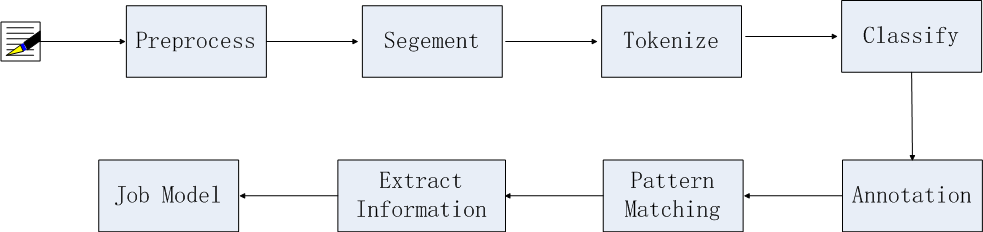
\includegraphics[scale=0.4]{images/pipeline.png}
  \caption{Job Description Process Pipeline}
  \label{fig:Pipeline}
\end{figure}


\section{Machine learning and Rule-based IE technologies}

There are two completive techniques in Information Extraction, one is machine learning-based approach, the other is rule-based approach. Chiticariu et al. \cite{chiticariu2013rule}summarized the pros and cons of machine learning (ML) and rule-based IE technologies in Table \ref{tab:mlrb}.

\begin{table}[ht]
\caption{Pros and Cons of ML and Rule-Based IE technologies } % title of Table
\centering % used for centering table
\begin{tabular}{ | c |  p{6cm} | p{6cm} | } % centered columns (4 columns)

\hline  %inserts double horizontal lines
 & Pros  & Cons  \\ [0.5ex] % inserts table
%heading
\hline % inserts single horizontal line
Rule-based &
    \begin{singlespace}
       \textbullet~Declarative  \par
       \textbullet~Easy to comprehend  \par
       \textbullet~Easy to maintain\par
       \textbullet~Easy to incorporate domain knowledge\par
       \textbullet~Easy to trace and fix the cause of errors  \par
    \end{singlespace}
    &  \begin{singlespace}
      \textbullet~Heuristic \par
       \textbullet~Requires tedious manual labor \par
       \end{singlespace}  \\
\hline
ML-based &
    \begin{singlespace}
       \textbullet~Trainable  \par
       \textbullet~Adaptable \par
       \textbullet~Reduces manual effort \par
    \end{singlespace}
    &  \begin{singlespace}
      \textbullet~Requires labeled data \par
       \textbullet~Requires retraining  for domain adaptation \par
        \textbullet~Requires ML expertise  to use or maintain \par
       \textbullet~Opaque  \par
       \end{singlespace} \\
\hline %inserts single line
\end{tabular}
\label{tab:mlrb} % is used to refer this table in the text
\end{table}

In this work, we prefer the rule-based approach because:
\begin{enumerate}
    \item Most of sentences that contain the information share some common patterns that can be easily identified.
    \item A lot of sentences are not grammatical completed as a sentence, for example some of them missing subject, and some of them are just a list of terms.
    \item Processing speed is also a concern, and generally rule-based approach is faster.
\end{enumerate}



\section{Semantic Label}

One conception always have similar but different expression, like Bachelor's degree, in job descriptions it could be written into bachelors degree, B.S., 4 years degree, and so on. In this work, we annotate words in the sentence with semantic label.

We create a dictionary which collect different spelling and expression to a concept. For example  Bachelor's degree has such dictionary entry.

["Baccalaureate","bachelors", "bachelor" ,"B.S.", "B.S","BS","BA","BA/BS", "BABS", "BSBA", "B.A." ,"4-year","4-year", "4 year", "four year","college","Undergraduate" , "University" ]

These words combining with following word ``degree'' will all have the same meaning. We know that the regular expression is a finite state machine (FSM), any word add into it, will become a state of the FSM. If we use common method, adding all these words into the regular expression, the matching process will meet problem of combinatorial explosion. Actually we don't care what the words the sentence use, we want to determine the if the words' meaning and category. So here we propose a two layers label approach. In the first level, we labeled the word with its semantic meaning, which is the value we want to extract from the sentence. In the second level, the labels are the semantic category of the first layer label. For example the word "bachelors" will be annotated in the first layer with label "BS LEVEL" which means bachelors degree level, and the word "PhD" will be labeled as "PHD LEVEL", the both be labeled with "DEGREE LEVEL" in the second layer. A labeled sentence is shown in ~\ref{tab:labeldsent}.

\begin{table}[ht]
\caption{Labeled sentence } % title of Table
\centering % used for centering table
\begin{tabular}{  | c | c | c | c | c |c | c |c | c | c |  }
 \hline
 layer 2 & DE LEVEL   & DEGREE & IN & MAJOR            & OR & MAJOR  &.  \\
 \hline
 layer 1 &  BS LEVEL   & DEGREE & IN & MAJOR CS         & OR & MAJOR INFO & .      \\
 \hline
   words & bachelors   & degree & in & computer science & or & information systems & .     \\
  \hline
\end{tabular}
\label{tab:labeldsent} % is used to refer this table in the text\section{Pipeline of Information Extraction}
\end{table}

\section{Regular Expression Over Labeled Tokens}

Cascaded Finite-State Transducers has widely used approach in Information Extraction for more than 20 years. This approach had been demonstrated   very effective in extracting information from text like CIRCUS~\cite{lehnert1991university} and FASTUS~\cite{hobbs199713}.  In the widely used NLP toolkit GATE~\cite{cunningham2002framework}, the semantic tagger JAPE (Java Annotations Pattern Engine) could describe patterns to match and annotations to be created as  a result. JAPE adopted a version of CPSL (Common Pattern  Specification Language)~\cite{appelt1998common}, which provides finite state transduction over annotations. Chang et al. presented cascaded regular expressions over tokens~\cite{chang2014tokensregex}, which proposed a cascaded patterns over token sequences.

After study these frameworks, I found most them are powerful, but complex. Developers need to learn some  domain-specific language (DSL) like CPSL, and how to integrate this part into a system will also bring some problem. So here we proposed a more flexible and lighter framework could do regular expression matching over labeled tokens.

The input of the pattern is sequence of array, every array is the token and its labels in different layer, which is showed in table~\ref{tab:labeldsent}. A pattern is a concatenation of matchers�� which is basic unit of the pattern. A matcher could match a token or a label in any layer.

Currently we support some types of matchers, we list them in table~\ref{tab:matchers}.  The framework support several styles to create a pattern, the most common one is regular expression style, like:

\begin{table}[ht]
\caption{Matcher Class } % title of Table
\centering % used for centering table
\begin{tabular}{  | l | l | l |  }
 \hline
 Class Name        &  Function                                 & Counter Part of regex    \\
 \hline
 UnitMatcher       &  token is matches the it                  & character  in regex       \\
 \hline
 SequenceMatcher   &  A list of Matcher                        & sequence of characters       \\
  \hline
 QuestionMatcher   &  One or more of the preceding token       & ?       \\
  \hline
 StarMatcher       &  Zero or more of the preceding token      & *       \\
  \hline
 PlusMatcher       &  Zero or one of the preceding token       & +       \\
  \hline
 DotMatcher        &  Any token                                & .      \\
  \hline
 RegexMatcher      &  Any token matches the regular expression               &        \\
  \hline

\end{tabular}
\label{tab:matchers} % is used to refer this table in the text\section{Pipeline of Information Extraction}
\end{table}

\begin{framed}
    \begin{lstlisting}[language=Python]
    seqMatcher =parser.parse(" aaa | bbb  ccc?  * ddd")
    \end{lstlisting}
\end{framed}

 The seconde style is use algebra operator to connect matchers, like this:

\begin{framed}
    \begin{lstlisting}[language=Python]
    seqMatcher =  TokenMatcher("aaa") +
           TokenMatcher("bbb") | TokenMatcher("ccc")
    \end{lstlisting}
\end{framed}

We also could create complex matcher in programming style, which just like we create some programming object, create some objects, and use them create a another object.

\begin{framed}
    \begin{lstlisting}[language=Python]
matcher1 = TokenMatcher("aaa")
matcher2 = TokenMatcher("bbb")
matcher3 = TokenMatcher("ccc")
matcher4 = AlternateMatcher([matcher1,matcher2])
seqMatcher = SeqMatcher([matcher3,matcher4])
    \end{lstlisting}
\end{framed}

We support these programming styles, because we want to give developers more flexibility to create patterns. The flexibility are come from the that developers could define which part of sequence should match by assign lambda expressions to matcher's catchfun and outfun. Since the every token in the sequence is an array, which is shown table~\ref{tab:labeldsent}, the lambda expressions could decide which field should be used to match, and which one should be outputed. For example,  to match the labeled sentence, the lambda expression for catchfun is "lambda x:x[2] ", and the outfun is "lambda x:x[1]", which means we match the pattern with the semantic category, and output the  the value we want. We show some patterns used to match degree in table:

\begin{table}[ht]
\caption{Patterns match degree} % title of Table
\centering % used for centering table
\begin{tabular}{  | l  |  }
 \hline
 DE\_LEVEL,  DE\_LEVEL, OR  DE\_LEVEL DEGREE   \\
 DE\_LEVEL DEGREE ( IN  $\vert$  OF ) DT MAJOR   \\
 MAJOR\_DEGREE  ,  MAJOR\_DEGREE OR MAJOR \\
 DE\_LEVEL (, DE\_LEVEL)* (OR DE\_LEVEL)? BE? PERFER\_VBD   \\
 \hline


\end{tabular}
\label{tab:patterns} % is used to refer this table in the text\section{Pipeline of Information Extraction}
\end{table}

\section{Implementation of Finite Automata Matching Library }

To transfer a token regular expression to a Finite Automata Transducers(FST), we need to steps: One is parsing  the expression to tree of structure of matchers, the other is transfer the tree of matchers to the Finite Automata Transducers.

We use PLY(Python Lex-Yacc) as the grammar parser, which  is a pure-Python implementation of the popular compiler construction tools lex and yacc. We defined  grammars of token regular expression in the parser, which can parse the token regular expression.

We use the algorithm proposed by Thompson and Ken\cite{thompson1968programming} to construct the FST from the tree. The expression like ``DL (, DL])*  (or DL)? DEGREE'' could be transferred to an FST in Figure ~\ref{fig:fst}.

\begin{figure}[htbp]
  \centering
  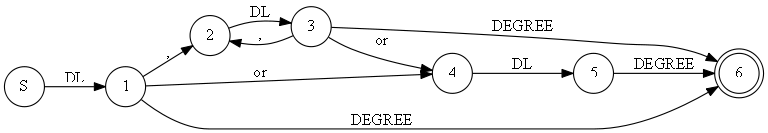
\includegraphics[scale=0.4]{images/test_tokenre2_6.png}
  \caption{Finite Automata Transducers}
  \label{fig:fst}
\end{figure}


